%%
%% IIVP 2026 report template
%%
\documentclass[a4paper,fleqn]{cas-sc}

\usepackage[authoryear]{natbib}

\usepackage{float}
\usepackage{amsmath}
\usepackage{booktabs}
\usepackage{graphicx}
\usepackage{multirow}

%%%Author definitions
\def\tsc#1{\csdef{#1}{\textsc{\lowercase{#1}}\xspace}}

\begin{document}

\graphicspath{{./}}

% Change your group number in both by replacing X!
\shorttitle{Group X}
\shortauthors{Group X}

% Change your group number in both by replacing X!
\title [mode = title]{IIVP2026 Group X Report}

% Change your names here for all member
% Replace StudentNameX with your full name. You can use spaces here.
% Replace studentidX with your student id. Only the digits. Do not put i or I at the beginning!
% Order of authors should be in alphebetical ordered by last name.
\author[1]{StudentName1}[orcid=studentid1]
\author[1]{StudentName2}[orcid=studentid2]
\author[1]{StudentName3}[orcid=studentid3]

% Do not change!
\affiliation[1]{organization={Department of Advanced Computing Sciences, Maastricht University},
            city={Maastricht},
            country={The Netherlands}}

% Do not change!!
\begin{abstract}
This report has been submitted for the KEN3238 - Introduction to Image and Video Processing course in Department of Advanced Computing Sciences at Maastricht University. The report is a requirement of the IIVP-2026 challenge. The challenge has been created by Dr. Yusuf Can Semerci and Dr. Gaurvi Goyal \citep{the_challenge}.
\end{abstract}

% Do not change!!
\begin{keywords}
KEN3238 \sep IIVP2026 \sep Hindi-MNIST \sep Digit Recognition
\end{keywords}
\maketitle 
\clearpage

% Your main text goes here!!!!
\section{Methodology}
Explain only your methodology using proper reference papers, algorithms, models and justifications.

You do not need to present your results or explain the problem presented to you through the challenge.


\bibliographystyle{cas-model2-names}
\bibliography{references}

\begin{figure}[h]
    \centering
    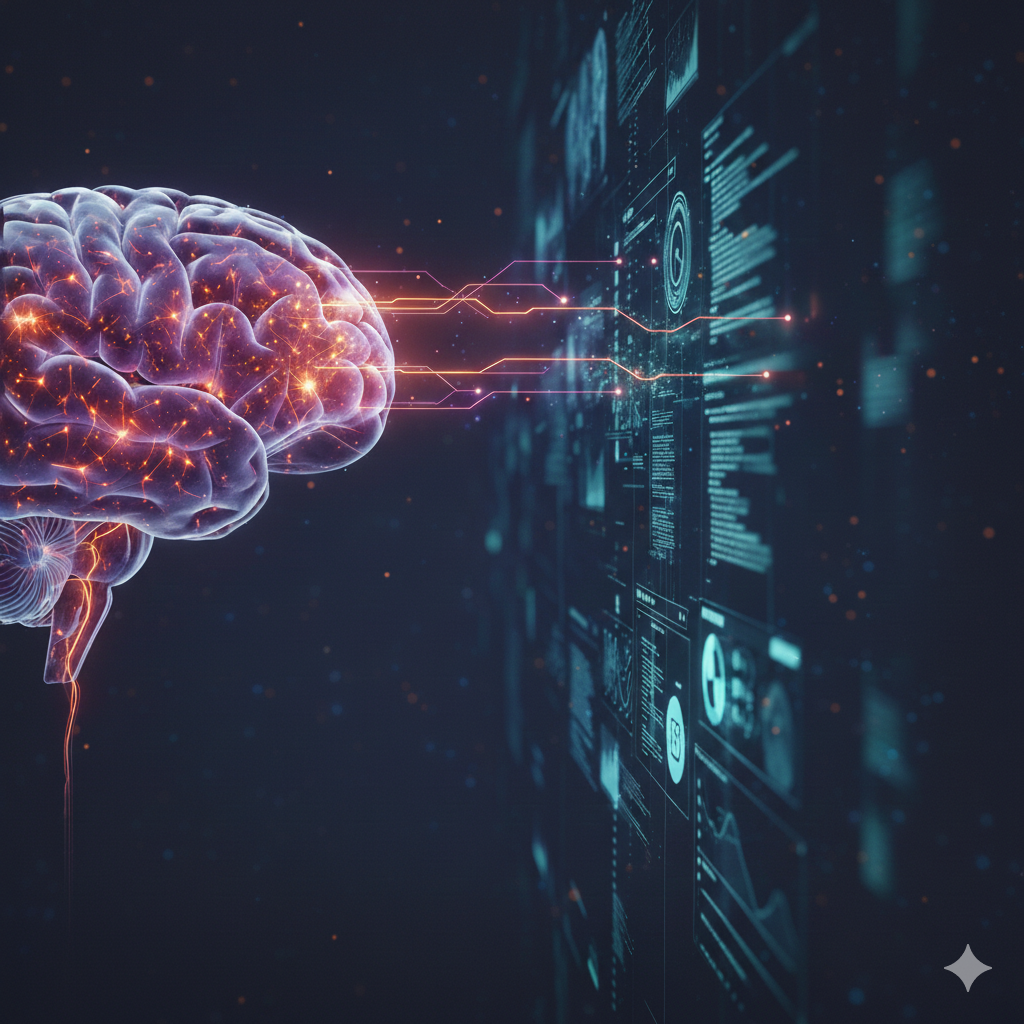
\includegraphics[width=0.4\linewidth]{Images/example.png}
    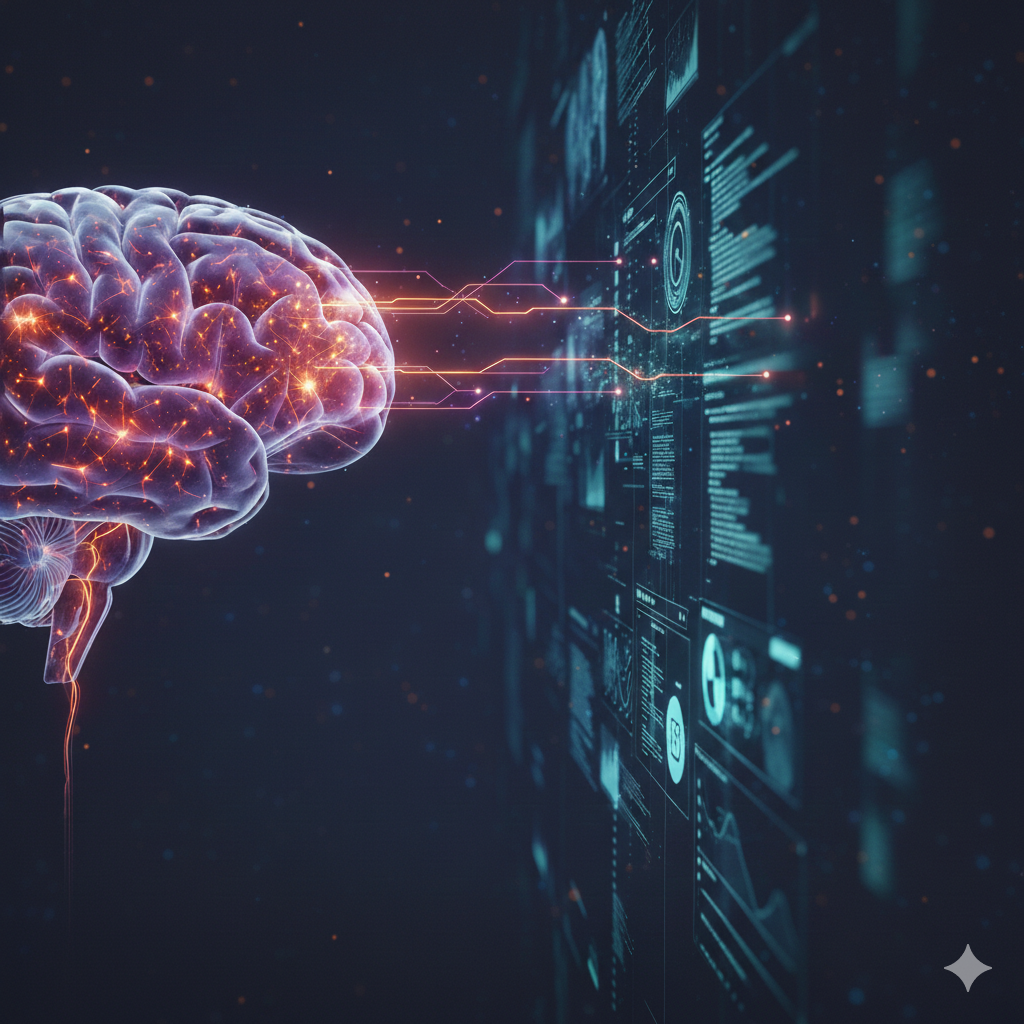
\includegraphics[width=0.4\linewidth]{Images/example.png}
    \caption{Example image left).. right)..}
    \label{fig:image}
\end{figure}
\begin{figure}[h]
    \centering
    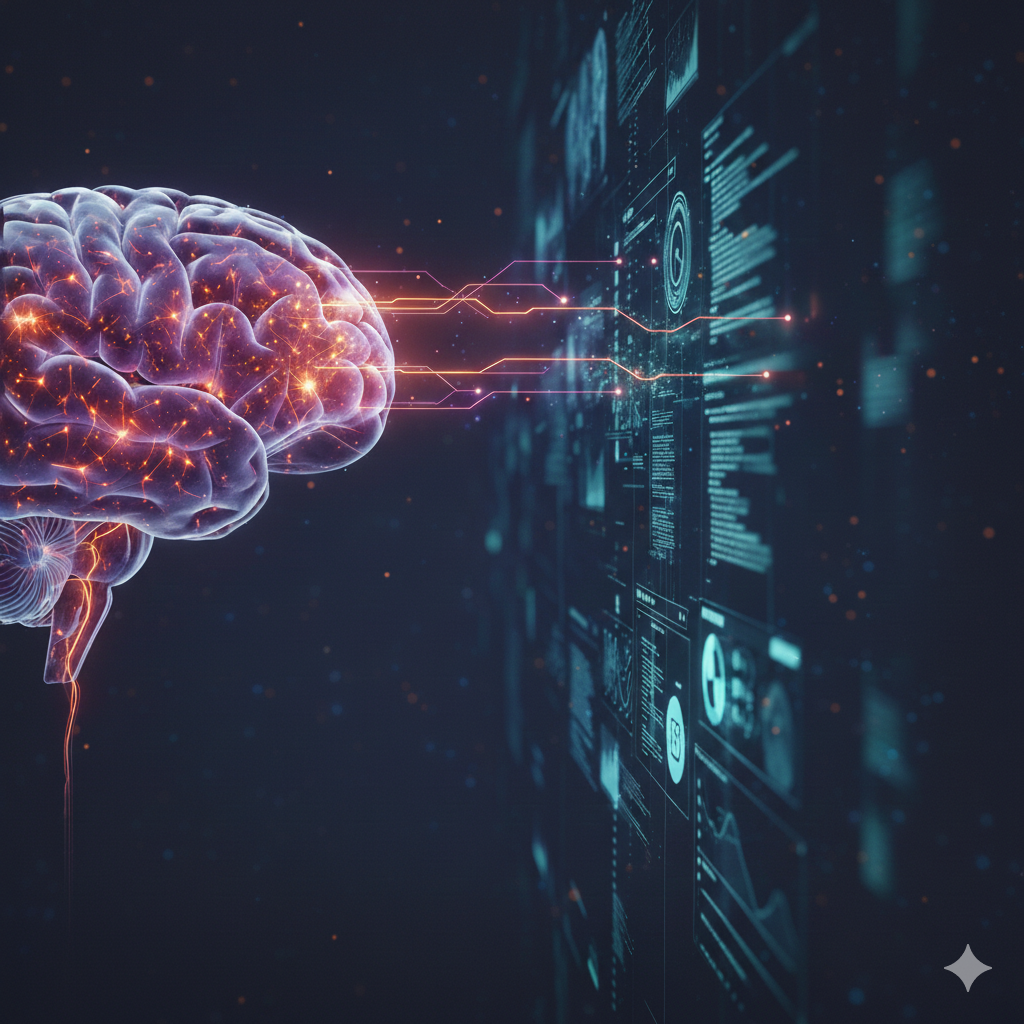
\includegraphics[width=0.4\linewidth]{Images/example.png}
    \caption{Example image}
    \label{fig:image}
\end{figure}

\end{document}
